% !TEX root = ../main_lecture_notes.tex
\chapter{Security of blockchain systems}\label{chap:security}
The security evaluation of blockchain systems consists in calculating the probability of a successful attack on the blockchain. We will focus, in \cref{sec:double_spending}, on the double spending attack which is concern for \PoW powererd cryptocurrency like teh bitcoin one. Security is also at risk when the node have an incentive to deviate from the prescribed protocol. \cref{sec:blockwithholding} discusses the opportunity for miner of \PoW equipped blockchain to resort to blockwithholding strategy to optimize their revenue. 

\section{Double-spending in PoW}\label{sec:double_spending}
A double spending attack aims at generating a concurrent blockchain to replace the main one. Consider the following scenario
\begin{enumerate}
	\item Marie sends to John BTC$10$
	\item The transaction from Marie to John is recorded in the blockchain
	\item John is advised for $\alpha$ confirmation, that is for $k-1$ block to be appended after the block where the Marie to John transaction is recorded
	\item Once $\alpha$ confirmations have been sent, John ships the good
	\item Meanwhile, Marie has started working on her own blockchain version where the Marie to John transaction is replaced by a Marie to Marie transaction
	\item At the shipment date the main blockchain is ahead by $z$ blocks 
	\item Marie's goal is then to work on her blockchain branch to catch up with the main branch. If she manages to to that then her branch will replace the public branch and she recovers her bitcoin. She can therefore spend these bitcoins again hence the name double spending.
\end{enumerate}
The race between the two competing branches of the blockchain is summarized on \cref{fig:dp_illustration}.
\begin{figure}[ht!]
\begin{center}
\begin{tikzpicture}[-, >=stealth', auto, semithick, node distance=1cm]
% \tikzstyle{block} = [rectangle, draw, fill=blue!20,
%     text width=5em, text centered, rounded corners]
\tikzstyle{block}=[rectangle, fill=black,draw=black,thick,text=black,scale=1.5]
\tikzstyle{block}=[rectangle, fill=white,draw=black,thick,text=black,scale=1.5]
\tikzstyle{confirmed block}=[rectangle, fill=white,draw=blue,thick,text=black,scale=1.5]
\tikzstyle{bad block}=[rectangle, fill=white,draw=red,thick,text=black,scale=1.5]
\node[block]    (1)                     {\tiny $\text{M}\rightarrow \text{J}$};
\node[block]    (2)[right of=1]                     {};
\node[block]    (3)[right of=2]                     {};
\node[block]    (4)[right of=3]                     {};
\node[confirmed block]    (5)[right of=4]                     {};

\node[bad block]    (6)[below of=1]         {\tiny $\text{M}\rightarrow \text{M}$};
\node[block]    (7)[right of=6]         {};
\node[block]    (8)[right of=7]         {};
\path
(1) edge[ left]     node{}     (2)
(2) edge[ left]     node{}     (3)
(3) edge[ left]     node{}     (4)
(4) edge[ left]     node{}     (5)
(6) edge[ left]     node{}     (7)
(7) edge[ left]     node{}     (8);

\end{tikzpicture}
\end{center}
\caption{Double spending race illustrated}
\label{fig:dp_illustration}
\end{figure}
\subsection{Random walk model}\label{ssec:double_spending_rw}
We define a discrete time stochastic process $(R_n)_{n\geq0}$ equal to the difference in length between the public and the private branch of the blockchain. At each time step a block is found, it belongs to the main branch with probability $p$ to the other branch with probability $q=1-p$. The parameter $p$ represents the proportion of hashpower owned by the honest miners, while $q$ is that of the attacker. We have
$$
R_0 = z\text{, and  }R_n = z+Y_1+\ldots+ Y_n.
$$
The $Y_i$'s are \iid random variables such that 
$$
\mathbb{P}(Y=1) = p\in (0,1)\text{, and }\mathbb{P}(Y=-1) = 1-p=q,
$$ 
$(R_n)_{n\geq0}$ is therefore a random walk on $\mathbb{Z}$. We assume that $p>q$ so that the attacker does not hold more than half of the total hashpower. Define the double spending time as 
$$
\tau = \inf\{n>0\text{ ; }R_n = 0\}.
$$
Our goal is to study the distribution of this stopping time with respect to the filtration 
$$
\mathcal{F}_n = \sigma(Y_1,\ldots, Y_n),\text{ }n\geq1.
$$ 
An illustration of this first-hitting time problem is provided in \cref{fig:double_spending_time}.
\begin{figure}[ht!]
\begin{center}
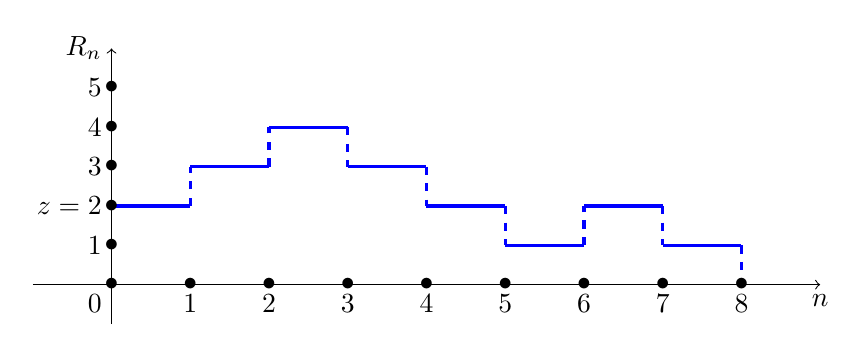
\begin{tikzpicture}
  %Origin and axis
  \coordinate (O) at (0,0);
  \draw[->] (-1,0) -- (9,0) coordinate[label = {below:$n$}] (xmax);
  \draw[->] (0,-0.5) -- (0,3) coordinate[label = {left:$R_n$}] (ymax);
  %Lower linear boundary

 
  %Stochastic process trajectory
  
  \draw (0,0) node[blue,left] {} node{};
  \draw[very thick,blue,-] (0,1) -- (1,1) node[pos=0.5, above] {} ;
  \draw[very thick,dashed,blue] (1,1) -- (1,1.5) node[pos=0.5, right] {};
  \draw[very thick,blue,-] (1,1.5) -- (2,1.5) node[pos=0.5, above] {};
  \draw[very thick,dashed,blue] (2,1.5) -- (2,2) node[pos=0.5, right] {};
  \draw[very thick,blue,-] (2,2) -- (3,2) node[pos=0.5, above] {};
  \draw[very thick,dashed,blue] (3,2) -- (3,1.5) node[pos=0.5, right] {};
  \draw[very thick,blue,-] (3,1.5) -- (4,1.5)node[pos=0.5, above] {};
  \draw[very thick,dashed,blue] (4,1.5) -- (4,1) node[pos=0.5, right] {};  
  \draw[very thick,blue,-] (4,1) -- (5,1) node[pos=0.5, above] {};
  \draw[very thick,dashed,blue] (5,1) -- (5,0.5) node[pos=0.5, right] {};  
  \draw[very thick,blue,-] (5,0.5) -- (6,0.5) node[pos=0.5, above] {};
  \draw[very thick,dashed,blue,-] (6,0.5) -- (6,1) node[pos=0.5, above] {};
   \draw[very thick,blue,-] (6,1) -- (7,1) node[pos=0.5, above] {};
    \draw[very thick,dashed,blue,-] (7,1) -- (7,0.5) node[pos=0.5, above] {};
     \draw[very thick,blue,-] (7,0.5) -- (8,0.5) node[pos=0.5, above] {};
     \draw[very thick,dashed,blue,-] (8,0.5) -- (8,0) node[pos=0.5, above] {};
  %Jump Times
  \draw (1,0) node[black,below] {$1$} node{ \color{black}$\bullet$};
  \draw (2,0) node[black,below] {$2$} node{ \color{black}$\bullet$};
  \draw (3,0) node[black,below] {$3$} node{ \color{black}$\bullet$};
  \draw (4,0) node[black,below] {$4$} node{ \color{black}$\bullet$};
  \draw (5,0) node[black,below] {$5$} node{ \color{black}$\bullet$};
  \draw (6,0) node[black,below] {$6$} node{ \color{black}$\bullet$};
  \draw (7,0) node[black,below] {$7$} node{ \color{black}$\bullet$};
  \draw (8,0) node[black,below] {$8$} node{ \color{black}$\bullet$};
  %Level of the counting process
   \draw (0,0) node[black,below left] {$0$} node{ \color{black}$\bullet$};
   \draw (0,0.5) node[black,left] {$1$} node{ \color{black}$\bullet$};
   \draw (0,1) node[black,left] {$z=2$} node{ \color{black}$\bullet$};
   \draw (0,1.5) node[black,left] {$3$} node{ \color{black}$\bullet$};
   \draw (0,2) node[black,left] {$4$} node{ \color{black}$\bullet$};
   \draw (0,2.5) node[black,left] {$5$} node{ \color{black}$\bullet$};

  % %Aggregated Capital gains
%  \draw (0,1.5) node[blue,below right] {$\mu_1$} node{ \color{blue}$-$};
%  \draw (0,2.25) node[blue,left] {$\mu_2$} node{ \color{blue}$-$};
%  \draw (0,3.75) node[blue,left] {$\mu_3$} node{ \color{blue}$-$};
  %Ruin time = First-crossing time time
%  \draw (5,0) node[black,above right] {$\tau_u$} node{ \color{black}$\times$};
%  \draw[dotted,black] (0,3.28) -- (5,3.28);
%  \draw[dotted,black] (5,0) -- (5,3.28);
\end{tikzpicture}
\end{center}
\caption{Illustration of the first-hitting time problem of a double spending attack.}
\label{fig:double_spending_time}
\end{figure}
\subsubsection{Double spending probability}\label{sssec:double_spending_rw_dsp}

\subsubsection{Double spending time}\label{sssec:double_spending_rw_dst}
\subsection{Counting process model}\label{sec:counting_process}
Let us denote by 
$$
\mathbb{P}_z(\cdot) = \mathbb{P}(\cdot|R_0 = z)\text{ and }\mathbb{E}_z(\cdot) = \mathbb{E}(\cdot|R_0 = z) 
$$
We are interested for now in the cvonditional distribution of $\tau$ provided that $R_0 = z$.
\subsubsection{Double spending probability}\label{sssec:double_spending_counting_process_dsp}
The double spending probability is defined as 
$$
\phi(z)=\mathbb{P}_z(\tau <\infty),
$$
and given in the following result
\begin{theo}
If $p>q$ then 
$$
\phi(z) = \left(\frac{q}{p}\right)^z.
$$
\end{theo}
\noindent We give two proofs for this result, the first one uses simple first step analysis exploiting the Markov property of the random walk. The second one uses Martingale and the optional stopping theorem.\\

\underline{\textit Proof 1:}\\
Using a first step analysis, we have 
\begin{equation}\label{eq:difference_equation}
\phi(z) = p\phi(z+1)+(1-p)\phi(z-1),\text{ }z\geq1.
\end{equation}
We also have the boundary conditions
\begin{equation}\label{eq:boundary_conditions_double_spending}
\phi(0) = 1\text{ and }\underset{z\rightarrow +\infty}{\lim}\phi(z) = 0
\end{equation}
Equation \eqref{eq:difference_equation} is a linear difference equation of order $2$ associated to the following characteristic equation
$$
px^2 - x + 1-p = 0
$$
which has two roots on the real line with 
$$
r_1 = 1, \text{ and }r_2 = \frac{1-p}{p}.
$$
The solution of \eqref{eq:difference_equation} is given by 
$$
\phi(z)=A+B\left(\frac{1-p}{p}\right)^z,
$$
where $A$ and $B$ are constant. Using the boudary conditions \eqref{eq:boundary_conditions_double_spending}, we deduce that
$$
\phi(z) = \left(\frac{1-p}{p}\right)^z
$$
as announced.\\
For the second proof we need the notion of martingale
\begin{definition}
A stochastic process $(X_n)_{n\geq0}$, is called a martingale with respect to a filtration $\mathcal{F}_n$, if
\begin{itemize}
	\item[(i)] $X_n$ is $\mathcal{F}_n$-adapted
	\item[(ii)] $\mathbb{E}(X_n)<\infty\text{ for }n\geq\geq0$ 
	\item[(iii)] $\mathbb{E}(X_n|\mathcal{F}_{n-1}) = X_{n-1}$
\end{itemize} 
\end{definition}
\noindent and the optional stopping theorem.
\begin{theo}
Let $T$ be a stopping time for the Martingale $(X_n)_{n\geq0}$ then it holds that 
$$
\mathbb{E}(X_T) = \mathbb{E}(X_0) 
$$
if there exists $c>0$ such that $|X_{T\land n}|<c$ for every $n>0$.
\end{theo}
\underline{\textit Proof 2:}\\
Define the process 
$$
X_n = \exp\left[s(R_n -z)- n\kappa_Y(s)\right],
$$
where $s>0$, and 
$$
\kappa_Y(s) = \log\left[\mathbb{E}\left(e^{sY}\right)\right],
$$
is the cumulant generating function of $Y$. 
\begin{lemma}\label{lem:wald_martingale_RW}
$(X_n)_{n\geq0}$ is a $\mathcal{F}_n$-martingale.
\end{lemma}
\begin{proof}
Denote by $M_Y(s) = \mathbb{E}(e^{sY})$ the moment generating function of $Y$, we have that 
\begin{eqnarray*}
\mathbb{E}(X_n|\mathcal{F}_n)&=&\mathbb{E}\left\{\exp\left[s(R_n -z)- n\kappa_Y(s)\right]|\mathcal{F}_n\right\}\\
&=&\exp\left[s(R_{n-1} -z)- n\kappa_Y(s)\right]\mathbb{E}\left[\exp\left(sY_{n}\right)|\mathcal{F}_n\right]\\
&=&\exp\left[s(R_{n-1} -z)\right]M_Y(s)^{-n} M_Y(s)\\
&=& X_{n-1}.
\end{eqnarray*}
\end{proof} 
The equation $\kappa_Y(s) = 0$ is equivalent to 
$$
pe^s+qe^{-s} = 1
$$
which admits $\gamma =\log(q/p)$ as only nonnegative solution. The process $(e^{\gamma R_n})_{n\geq0}$ is a $\mathcal{F}_n$-Martingale. Then applying the optional stopping theorem leads to 
$$
\mathbb{E}(X_\tau) = z\Leftrightarrow 
$$




\subsubsection{Double spending time}\label{sssec:double_spending_counting_process_dst}

\section{Blockwitholding in PoW}\label{sec:blockwithholding}
\subsection{The selfish mining strategy}\label{ssec:selfish_mining}
\subsection{Ruin and expected profit of a miner}\label{ssec:selfish_mining}
\subsection{Ruin and expected profit of a selfish miner}\label{ssec:selfish_mining}

\section{Nothing-at-stake in PoS}\label{sec:NaS}
\newpage